\documentclass[a4paper]{article}
\usepackage{multicol}
\usepackage{url}
\usepackage{graphicx}

\usepackage{amssymb}
\textheight 9.0in
\columnsep 0.375in
\textwidth 6.0in
\footskip 0.0in
\topmargin -0.0625in
\headheight 0.0in
\headsep 0.0in
\oddsidemargin 0.2in 
\parindent 0pc

\pagestyle{empty}
\newtheorem{sample}{Sample}

\begin{document}
\date{}
\title{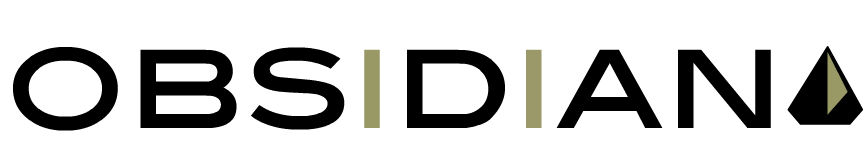
\includegraphics[scale=0.5]{../resources/images/logo_1.png}\textbf{\\}\textbf{\\}\Large \textbf{OBSIDIAN 0.1 DOCUMENTATION
\\}\vspace{0.5cm}}
\author{\textbf{Clement Game}\\clement(at)digi-nation(dot)com}

\maketitle
\thispagestyle{empty}

\vspace{3cm}
\begin{figure}[h]
\begin{center}
\label{fig:orga}
\end{center}
\end{figure}

\clearpage

{\textbf{This paper is released under the CC-by-SA licence.}
{\small\em }}
\vspace{0.5cm}
{\bf\it \\Keywords:}
{\small Peer-to-Peer,Fast R�plication,mirroring,Dexp,Linux }

\tableofcontents

\textbf{\\ \\ \\ \\}

\thispagestyle{plain}


\section{Introduction}

In ancient times, People was using a volcanic stone, which amount of 

Durant l'antiquiti�, les premiers premiers mirroirs concus par l'homme etaient fabriqu� � partir d'une pierre

\section{Overview}

Obsidian is a fast-mirroring, Peer-to-Peer software which was specially designed to maintain large file repositories synchronized with each others, featuring very fast changes propagating. \\\\To achieve this, Obsidian use 2 core technologies: Filesystem Events Listening , and a new protocol specially designed for the occasion: DEXP, acronym for Documents EXchange Protocol. With DEXP, Change Notifications are sent directly to the mirroring peers, so they don't have to poll periodically for file changes.\\\\

To illustrate how fast is Obsidian compared to a classical multiple rsync-based system, let's consider a chain of n peers, each node being synchronized to the next with a periodical rsynch check $(T_c)$.The time taken by each node to download a change is $T_d$.
In this case, the worst-case propagating time will be:\\\\

$ T_r = \sum_0^n T_d(n) + T_c(n) $\\\\
As we can see in this case (rsync) , the more nodes we have, the more time it loses, because of the accumulation the $T_c$ components.\\\\But in the other case (Obsidian) , the calculation of the maximum propagating time between n nodes is:\\\\
$ T_r  = \sum_0^n T_d(n) $\\\\
So with obisidan, The more nodes you haves, the more efficient it is compared to a periodic-poll based method. If we now consider a $T_c$ constant for each node, we can evaluate the speed gain with:\\\\ $T_g = nT_c$ \\

\section{Global Architecture}

This section explains how Obsidian works from a global point of vew:\\\\

Obsidian nodes are logically grouped by what we call 'Spheres of influence'. Each Obsidian node inside a sphere of influance receive the same announces, 
and all the nodes will end-up hosting the same files database.
 
2 distinct spheres of Influence appear when nobody belonging to sphere 1 has a peering connection to anybody Belonging to sphere 2   

\begin{center}
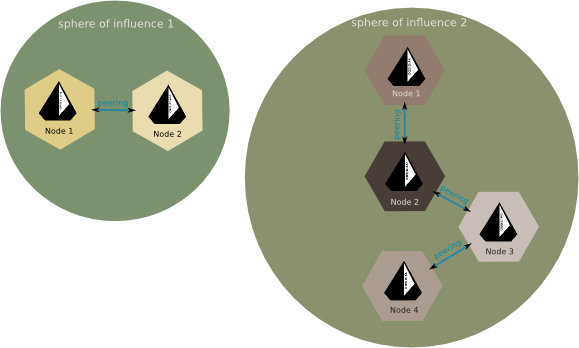
\includegraphics[scale=1]{../resources/images/global_arch_1.png}
\end{center}
Now let's make the model evolve. Node 2 from sphere 1 peers with node 2 from sphere 2: Since These 2 nodes will share announces, the 2 spheres will merge. 

\begin{center} 
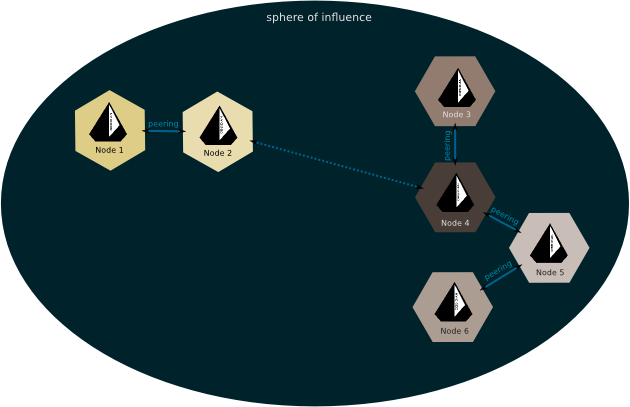
\includegraphics[scale=1]{../resources/images/global_arch_2.png}
\end{center}

From an ensemblist point of view, to describe the nodes behaviours while peering, we can write the following axioms:\\\\
$
n1 \epsilon S1 \\
n2 \epsilon S2 \\
peering(n1,n2) =>  n1 \epsilon (S1 \cup S2) ; n2 \epsilon (S1 \cup S2)\\\\$


\clearpage
\section{Software Architecture}

The Software architecture behind Obsidian is quite easy, and can be described with the following scheme:\\\\

\begin{center}
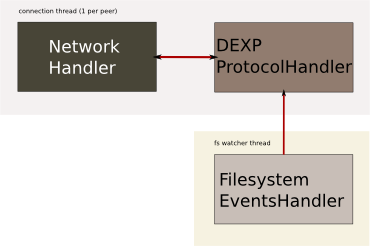
\includegraphics[scale=0.5]{../resources/images/software_arch.png}
\end{center}

Obsidian uses a multi-threaded architecture along with blocking sockets. This is probably the less efficient part of the software, 
because this model is very expensive, but this way it was was really quick to prototype something that works.\\
A futur version of obsidian will surely come with a fully asynchronous model, at least for connections handling, 
as soon as we'll have time to redesign it. \\\\

Obsidian makes use of two other threads: a watchdog for current connections, and the filesystem events handler.

\section{Getting Started with Obsidian}
This section describes in detail how to get started with Obsidian, step-by-step and from scratch.
\subsection{prerequisites}

In order to build and run Obsidian, you'll need: \\\\

- A GNU/Linux Op�rating System, with kernel 2.6.19 or higher.\\
- The OpenSSL Library plus its headers (libssl-dev) , 0.9.8 or higher.\\
- Cross-platform make (cmake 2.6 or higher).\\
- The GNU C compiler ( gcc-4.X ).\\
- Git DVCS(to retrieve the source code, if not done yet )\\\\

Also please note that you'll need root credentials on your system in order to install Obsidian. 

\subsection{Fetching the sources}

Here we're assuming that that you haven't fetched the obsidian source code yet. To do that, you will need the GIT DVCS, a well-known .

Once you have git installed on your system, just type:\\
 
\verb|$git clone git://github.com/digination/obsidian.git |


\subsection{Compilation}

This step explains how to build Obsidian from sources, with the use of cmake and gcc.

\subsubsection{Producing the Makefile}

This is cmake's duty to help you create a correct Makefile, suitable for your platform (even though up to know, obsidian is only compatible with Linux :P).\\
In order to produce your Makefile, you'll just have to use the following command at the root of obsidian's project tree :\\

\verb|$cmake -DCMAKE_INSTALL_PREFIX=/usr/local/obsidian . |\\

Also note that you can of course change the directory where obsidian will be installed, by modifying the CMAKE\_INSTALL\_PREFIX variable in the command above.

\subsubsection{Let's roll, baby !}

Now that the Makefile for obsidian has been created, we can lunch the actual compilation step, with the command:\\

\verb|$make |\\

\subsection{Installation}

Ok now that the compilation process is ok, let's install obsidian on the Syst�me, according to the PREFIX variable declared earlier.To install Obsidian, 
Nothing is more simple. From the Obsidian project Root Directory, just type the following: (as root)\\

\verb|$make install |\\

\subsection{Basic Configuration} 


\section{Configuration File} 

This section makes an exhaustive �numeration of all the options which can be modified inside obsidian's configuration file.

\subsection{Peers}

\subsection{Sockets/ Connection Options}

\subsection{TLS Options}

 
\section{Advanced Usages}

\subsection{Setting up TLS on your obsidian Server}

\subsection{Running multiple sessions of Obsidian on the same server}

In order to circumvence the zero-dir limitation, you can choose to run multiple instances of obsidian at the same time on your server, so your peers can replicate data from the multiple instances.

\section{More on DEXP}

This section explains in details how the underlying protocol created for obsidian,DEXP, actually works.

\subsection{A few notes to start}

\subsubsection{Client/Server relationship}

Like every Peer-to-Peer protocol, Obsidian acts both as a server for some peers, and as a client for others, and so there is no distinction between binaries, there's only "obsidian".

\subsubsection{Structure}

DEXP is mainly a text-based protocol, as can be HTTP, FTP, IMAP and many more; meaning that it's based on a specific, human-readable vocabulary.

\subsection{Steps}

Here we will describe in a detailed way the differents step of a DEXP session, from the beginning. 

\subsubsection{Connection}



\subsubsection{Capacities}

Once the TCP session has been established between two obsidian servers, the peer acting as a server will sent its capacities, consisting of a set of informations allowing the session between the two peers to be correctly negotiated.\\
These informations are:\\\\

   
 

\subsubsection{Session Negotiation}

Once the server sent its capacities to the client, the client will then choose which protocol version to use, comparing the received protocols list to its own one,
choosing the higher matching one. The the protocol version is choosen, the client will send a "NEGOTIATE" command followed by the protocol version it choose, as argument.

\subsubsection{TLS Negotiation (optionnal)}

If the server announced TLS capacities, the client will systematically try to negotiate a TLS session with its peer, 
using a "STARTTLS" command (like many other protocols, doing the same ). If TLS is correctly configured on the server,
the negotiation will completed and the trafic between the two peers will then be ciphered.

\subsubsection{Catalogs Exchange and files Synchronisation (optionnal)}

Once the session and security layer have been negotiated, the client will start sending it's own files catalog to the host 


\subsubsection{Announces propagation}
 
\subsubsection{Files transferts}

\subsubsection{Announces delaying}

If an announce has to be sent to a peer but this peer is currently busy sending or receiving data, the announce is placed in a queue and sent once the peer becomes
available again. a peer notices its availability by sending a "READY" command to the server it was previously sending/receiving data to/from.

\section{Known Bugs, Limitations}

There is no knwon bug at this time, but the situation will change for sure.\\
Also the main limitation of Obsidian the "zero-dir" issue, meaning that it's filesystem events handler cannot detect changes located in subdirectories located inside the data\_dir. That's why, for now, Only the root of the data directory will be replicated. (subdirectories are simply ignored).\\ 
This is the main change expected for version 0.2: A recursive fs events handler.

\section{Special Thanks}

My special thanks go to "Le Loop" Hackerspace in Paris and their fellow members, for providing me their support, advices and a place to crash and work on my project.

\end{document}
